\subsection{Flip angle optimisation}
\label{subsec:pureshift__faopt}

Having described the rest of the optimisation setup, it remains to choose exactly which parameters are subjected to optimisation.
The simplest option is to only optimise one parameter, namely the flip angle of the (double-)saltire pulse.
The flip angle dependence of PSYCHE spectra is well-understood, which crucially allows us to evaluate the cost functions outlined above and determine whether they are functioning correctly.

\begin{figure}[htb]
    \centering
    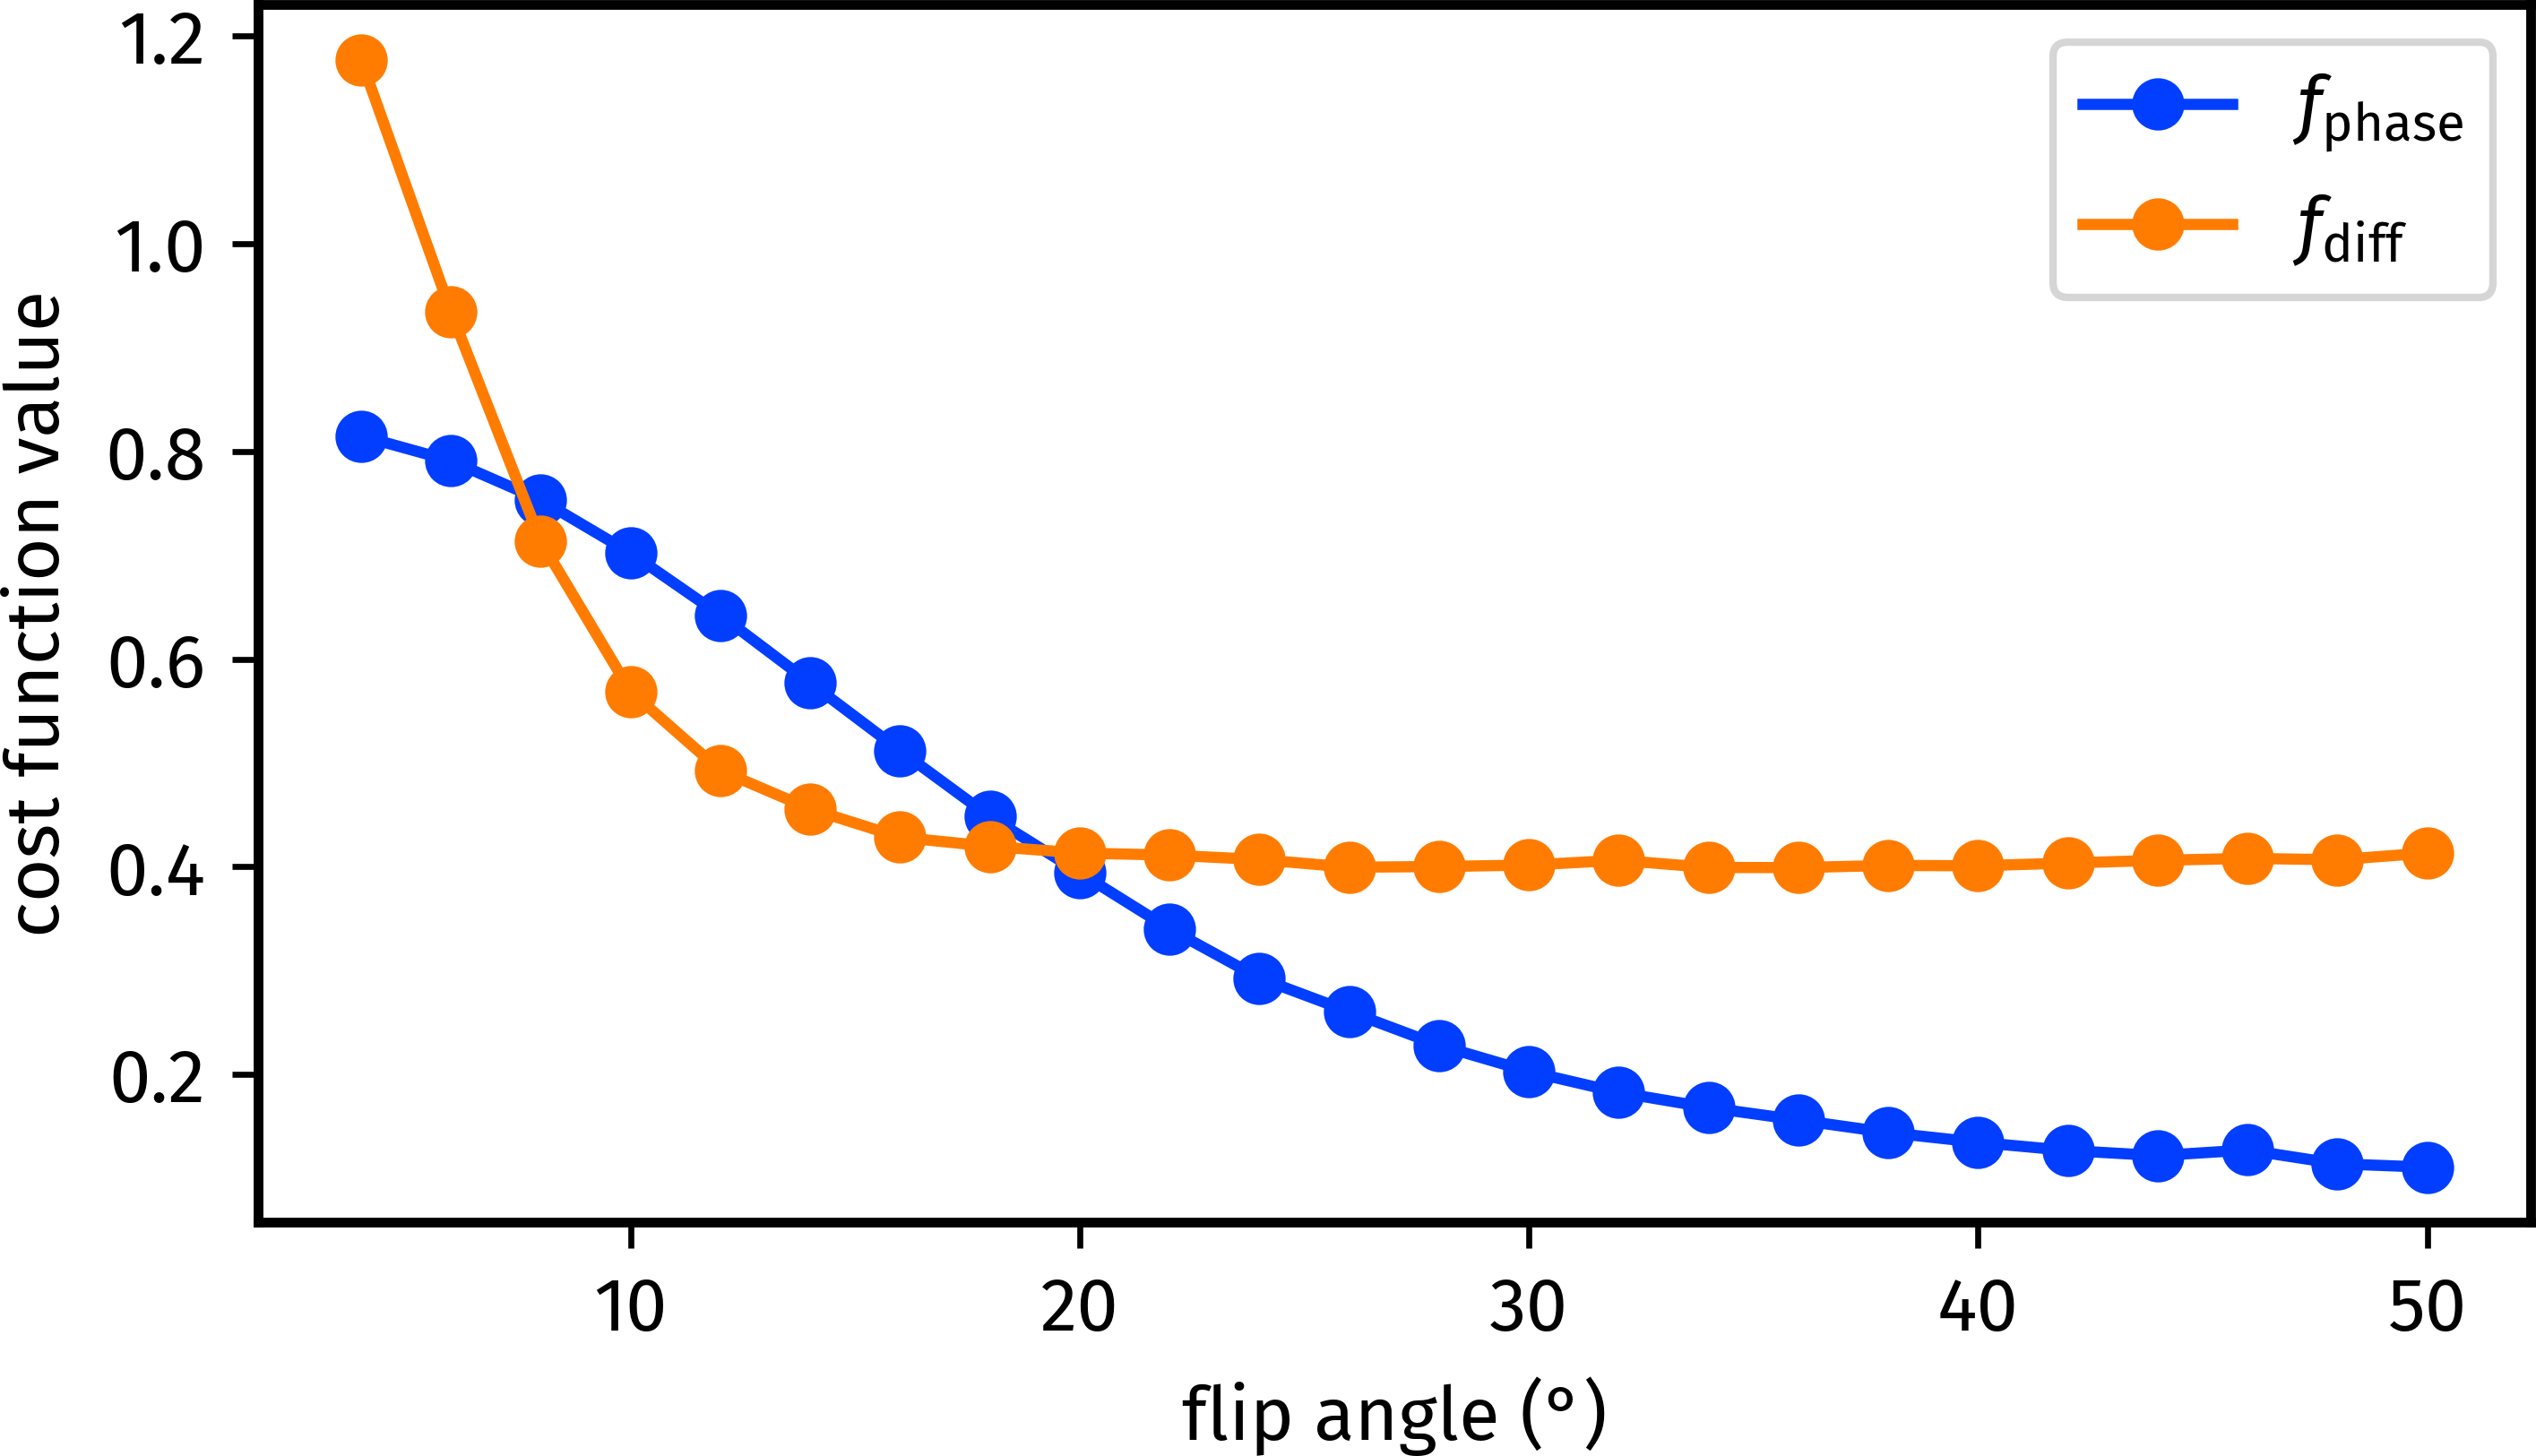
\includegraphics[]{pureshift/fa_scan_cyclo.png}%
    \caption[Behaviour of $f_\text{phase}$ and $f_\text{diff}$ on experimental J-refocused spin echo spectra.]{
        Behaviour of the two cost functions, $f_\text{phase}$ and $f_\text{diff}$, on experimental J-refocused spin echo spectra.
        \datacode{5C-190809}
    }
    \label{fig:fa_scan_cyclo}
\end{figure}

I first sought to measure how the cost functions described above varied with the flip angle.
To this end, JRSE spectra using a \textit{single} saltire as the PSE and various flip angles (from \ang{10} to \ang{50}) were acquired (\cref{fig:fa_scan_cyclo}).
Since both cost functions penalise both low sensitivity and low purity, we might expect that there is be an intermediate value where neither sensitivity nor purity were penalised too much: this would the `optimum' flip angle.
In the event, it was found that only $f_\text{diff}$ yielded a useful---albeit shallow---minimum at around \ang{25} (recall that the PSE here is a single saltire, so this corresponds roughly to a \ang{15}--\ang{20} double saltire).
The $f_\text{phase}$ cost function, on the other hand, was strictly decreasing within the range of flip angles tested: it is possible that there is an optimum at an even larger flip angle, but this would have been a scientifically unsound conclusion given that the sample was decently concentrated (\qty{50}{\milli\molar}).

This naturally raises the question of why $f_\text{diff}$ yields an optimum which falls within what we would consider a `sensible' region.
It is tempting to believe that the form of $f_\text{diff}$ (\cref{eq:ps_cf_diff}), which is at first glance quite intuitive, naturally leads to a better result.
I argue here, however, that this is mostly down to \textit{coincidence}.
This is difficult to explain quantitatively, but in a broader sense, we may imagine that the cost function separately penalises low sensitivity and low purity, i.e.\ it can be decomposed into something of the form
\begin{equation}
    \label{eq:cost_function_generic}
    f = g(s) + \lambda h(p),
\end{equation}
where $s$ and $p$ are respectively the sensitivity and purity, and $g$ and $h$ are some unknown functions which \textit{decrease} with increasing $s$ and $p$ (since we want to minimise the cost function).
This is clearly a simplification, because the plots in \cref{fig:fa_scan_synthetic} show that the effects of sensitivity and purity on the cost functions are not additive; however, it is sufficient to make the point here.
The parameter $\lambda$ represents the relative weighting of purity to sensitivity: if $\lambda$ is large than the purity is more strongly emphasised, and vice versa if $\lambda$ is small.

When we say that an optimum is `sensible' or `sound', this is with respect to the sensitivity/purity balance in the parent pseudo-2D homodecoupled spectrum.
In other words, what we \textit{really} seek is a cost function which measures the sensitivity and purity of that spectrum:
\begin{equation}
    \label{eq:cost_function_generic_p2d}
    f' = g'(s') + \lambda' h'(p'),
\end{equation}
where everything is marked with a prime symbol to indicate that it is with respect to the decoupled spectrum, and the parameter $\lambda'$ is chosen to fit our judgement of the required balance, or in other words, yield an optimum of around \ang{20}.
Now, we may reasonably assume that $s$ and $s'$ are proportional, but $p$ and $p'$ are hardly the same thing: one is manifested in terms of artefact intensity and the other in terms of phase distortions.
Furthermore, the $\lambda$ provided to us by the cost function $f$ may not necessarily be the same as our ideal choice of $\lambda'$; let alone the forms of the functions $g$ and $h$.
The fact that \cref{eq:cost_function_generic} \textit{happens} to provide the same flip angle optimum as the idealised \cref{eq:cost_function_generic_p2d} cannot truly be attributed to design!

Of course, just because a cost function works mostly by serendipity does not mean that it cannot be used.
    So, I ran several \textit{actual} optimisations of the flip angle using the cost function $f_\text{diff}$, which reliably converged to optima between \ang{20} and $\ang{25}$ regardless of the initial point chosen.
Typically, around 10 spectrum acquisitions were required, corresponding to a time of around 2--4 minutes.
This is not surprising in light of our knowledge of $f_\text{diff}$; however, it provides us with a proof-of-principle that automated optimisation of NMR parameters is possible.
Further optimisations of the PSYCHE flip angle are also discussed in \cref{subsec:poise__psyche}.
